\documentclass{beamer}
\usetheme{metropolis}  
%\setbeamertemplate{frame footer}{Rebecca Eifler}
%\setbeamertemplate{footline}[frame number]
\usepackage{appendixnumberbeamer}
\usepackage[english]{babel} 
\usepackage{listings}
\usepackage{xcolor, colortbl}
\usepackage[inference]{semantic}
\usepackage{tikz}
\usetikzlibrary{arrows,automata,shadows, shapes, positioning}
\usepackage{pgf-umlsd}
\usepackage{pgfplots}
\usepackage{hyperref}
\usepackage{mathtools}
\usepackage{stmaryrd}
\usepackage{ upgreek }
\usepackage{ marvosym }
\usepackage{tabularx}
\usepackage{booktabs}
\usepackage{algpseudocode}
\usepackage{subcaption}
\usepackage{marvosym}
\usepackage{varwidth}

\newcommand{\image}[1]{
	\includegraphics[scale=0.06]{images/image#1.png}
}


\newcommand{\samerover}[2]{
	\begin{tikzpicture}
		\node[] (r1) at (-0.7,0) {
\includegraphics[scale=0.04]{images/rover1.png}};
		\node[] (xor) at (0.05,0) {$\otimes$};
		\node[] (r2) at (0.7,0) {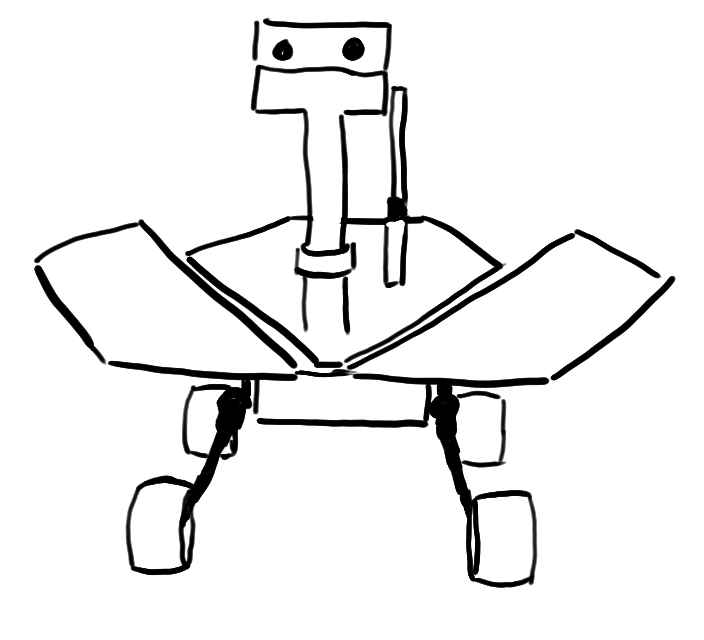
\includegraphics[scale=0.04]{images/rover2.png}};
		\node[] (i1) at (-0.5,1) {\includegraphics[scale=0.06]{images/image#1.png}};
		\node[] (i2) at (0.5,1) {\includegraphics[scale=0.06]{images/image#2.png}};
		\node[] (n) at (0,-0.7) {same rover};
	\end{tikzpicture}
}


\newcommand{\energylimit}[1]{
	\begin{tikzpicture}
		\node[] (i1) at (0,1) {\includegraphics[scale=0.06]{images/image#1.png}};
		\node[] (i2) at (-0.5,0) {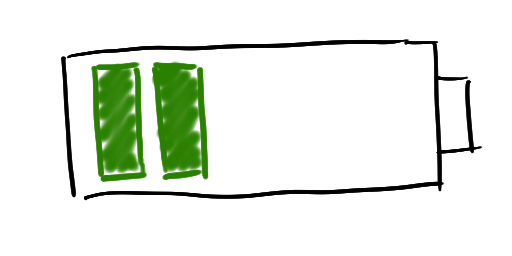
\includegraphics[scale=0.06]{images/battarie_low.png}};
		\node[] (p) at (0.8,0) {\large $> 50\%$};
		\node[] (n) at (0,-0.7) {energy limit};
	\end{tikzpicture}
}

\newcommand{\orderprop}[2]{
	\begin{tikzpicture}
		\node[] (i11) at (-0.5,1.2) {$1.$};
		\node[] (i1) at (-0.5,0.5) {\includegraphics[scale=0.06]{images/image#1.png}};
		\node[] (i11) at (0.5,1.2) {$2.$};
		\node[] (i2) at (0.5,0.5) {\includegraphics[scale=0.06]{images/image#2.png}};
		\node[] (n) at (0,-0.7) {order};
	\end{tikzpicture}
}


\newcommand{\specificrover}[2]{
	\begin{tikzpicture}
		\node[] (r1) at (0,0) {\includegraphics[scale=0.05]{images/rover#1.png}};
		\node[] (i2) at (0,1) {\includegraphics[scale=0.06]{images/image#2.png}};
		\node[] (n) at (0,-0.7) {specific rover};
	\end{tikzpicture}
}


\newcommand{\useconnection}[3]{
	\begin{tikzpicture}
		\node[] (r1) at (0,0.3) {\includegraphics[scale=0.05]{images/rover#1.png}};
		\node[draw, circle, inner sep=1pt] (Lx) at (-1,-0.5) {\small $L_#2$};
		\node[draw, circle, inner sep=1pt] (Ly) at (1,-0.5) {\small $L_#3$};
		\draw[thick, <->] (Lx) to (Ly);
		\node[] (n) at (0,-1) {use connection};
	\end{tikzpicture}
}


\newcommand{\dontuseconnection}[3]{
	\begin{tikzpicture}
		\node[] (r1) at (0,0.3) {\includegraphics[scale=0.05]{images/rover#1.png}};
		\node[] (r1) at (0,-0.45) {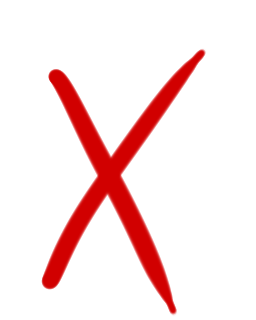
\includegraphics[scale=0.08]{images/no.png}};
		\node[draw, circle, inner sep=1pt] (Lx) at (-1,-0.5) {\small $L_#2$};
		\node[draw, circle, inner sep=1pt] (Ly) at (1,-0.5) {\small $L_#3$};
		\draw[thick, <->] (Lx) to (Ly);
		\node[align=center] (n) at (0,-1.1) {don't use\\[-0.3cm]connection};
	\end{tikzpicture}
}


\newcommand{\energylimitloc}[1]{
	\begin{tikzpicture}
		\node[] (r1) at (0,0) {\includegraphics[scale=0.05]{images/rover#1.png}};
		\node[] (b1) at (-0.5,1) {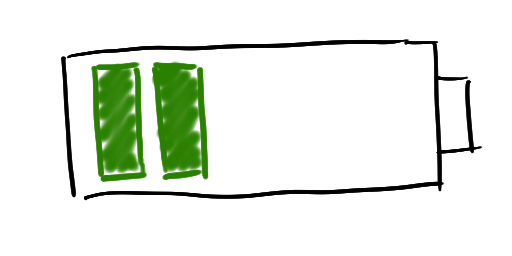
\includegraphics[scale=0.06]{images/battarie_low.png}};
		\node[draw, circle, inner sep=1pt] (l) at (0.5,1) {$L_y$};
		\node[] (n) at (0,-0.7) {energy limit};
	\end{tikzpicture}
}


\newcolumntype{L}[1]{>{\raggedright\arraybackslash}p{#1}}
\newcolumntype{C}[1]{>{\centering\arraybackslash}p{#1}}
\newcolumntype{R}[1]{>{\raggedleft\arraybackslash}p{#1}}

\definecolor{darkgreen}{HTML}{009900}
\definecolor{mBlue}{HTML}{005CE6}

% beamer uncover for row colors
\makeatletter
\def\rowcolor{\noalign{\ifnum0=`}\fi\bmr@rowcolor}
\newcommand<>{\bmr@rowcolor}{%
	\alt#1%
	{\global\let\CT@do@color\CT@@do@color\@ifnextchar[\CT@rowa\CT@rowb}% 
	{\ifnum0=`{\fi}\@gooble@rowcolor}% 
}

\newcommand{\@gooble@rowcolor}[2][]{\@gooble@rowcolor@}
\newcommand{\@gooble@rowcolor@}[1][]{\@gooble@rowcolor@@}
\newcommand{\@gooble@rowcolor@@}[1][]{\ignorespaces}
\makeatother


\newcommand\Wider[2][3em]{%
	\makebox[\linewidth][c]{%
	  \begin{minipage}{\dimexpr\textwidth+#1\relax}
		\raggedright#2
	  \end{minipage}%
	}%
}


%\setbeamertemplate{section in toc}{\textbf{\inserttocsection}}
%\setbeamertemplate{frame footer}{Rebecca Eifler}

\title{Explaining the Space of Plans through Plan-Property Dependencies\vspace*{-0.6cm}}
\author{Rebecca Eifler}
\date{15.03.2019}
%\institute{Foundations of Artificial Intelligence}
\institute{\vspace*{0cm}\hspace*{7cm}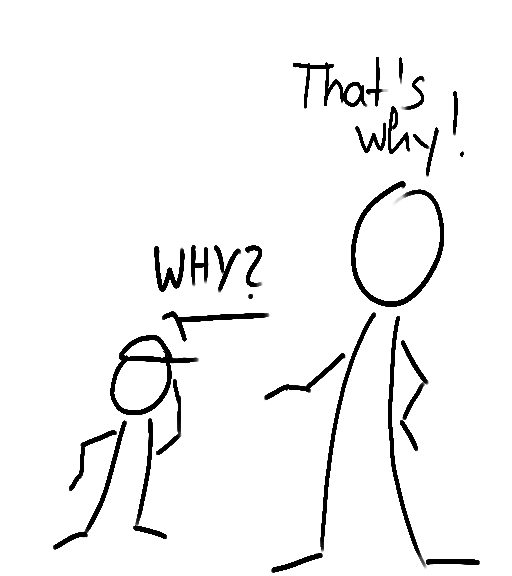
\includegraphics[scale=0.25]{images/warum_darum.png}}
\titlegraphic{\vspace*{5.5cm}\hspace*{-0.5cm}
\includegraphics[scale=0.25]{logo_grad_school}}


\begin{document}
\metroset{block=fill, progressbar=frametitle}
%\setbeamertemplate{frame footer}{Rebecca Eifler}

\maketitle

\section{Introduction}
\label{introduction}

AI plan generation technology serves to generate a plan $\pi$ based on
a world model. If the model and optimization objective reflect the
real world and user preference with absolute accuracy, then $\pi$ can
be executed as-is. Yet in many usage scenarios, that is not so. Often,
models are approximate, optimization objectives are highly complex
and/or implicit in the heads of the human users, and bad plan
decisions can be highly detrimental. A prominent example are space
applications as discussed \eg\ by Smith \shortcite{smith:aaai-12}, but
arguably also many other applications ranging from Industry 4.0 to
robot-aided disaster recovery. As Smith pointed out, planning should
then be an iterative process in which the planning system suggests
plan candidates, to be inspected and criticised by human users for
iterative plan improvement.

As Smith also pointed out, plan explanation is a crucial step of such
an iterative process, as a key means for user inspection. In
particular, questions of the form ``Why does the plan not achieve goal
$G$?'' or ``Why don't you satisfy preference $P$?'' need to be
answered. Such answers require insights about the space of possible
plans. We propose to address this by \defined{plan-property
  entailments}, as in ``Because achieving $G$ would necessitate to
either forego $G'$ or use $> 100$ energy units''. More formally, a
plan property $p$ is a Boolean function on plans (\eg\ $G$ true at
end), and $p$ entails $q$ if all plans that satisfy $p$ also satisfy
$q$.  A user question of the form ``Why not $p$?'' can then be
answered in terms of those $q$ entailed by $p$ (\eg\ $G'$ false at end
or energy usage $> 100$). We will refer to this as a \defined{local}
explanation, in difference to the \defined{global} explanation showing
the graph of all plan-property entailments. The former makes sense in
iterative planning as outlined; the latter makes sense when an
overview of plan space is desirable, for example in simulated
penetration testing \cite{boddy:etal:icaps-05,hoffmann:icaps-15} where
system security may be best facilitated by a global view on the space
of possible attacks.
%
%% Moreover, the graph of all plan-property entailments provides an
%% overview explanation of plan space. We will refer to the latter as a
%% \defined{global} explanation, and to the answer to a specific user
%% question as a \defined{local} explanation.
%% %
%% An example use case for global explanations is simulated penetration
%% testing \cite{boddy:etal:icaps-05,hoffmann:icaps-15}, where system
%% security is best facilitated by a global view on the space of possible
%% attacks.
  
Our form of plan explanation falls into the class of
\emph{contrastive} explanations as discussed \eg\ by Miller
\shortcite{miller:ai-19}. Previous work on local explanation, \ie,
answering questions of the form ``Why not $p$?'', has suggested to
generate a new plan $\pi'$ that satisfies $p$, and answer the question
based on comparing $\pi$ and $\pi'$
\cite{smith:aaai-12,fox:etal:ijcai-ws-17}. A weakness of this idea is
that there may be differences between $\pi$ and $\pi'$ unrelated to
$p$. Our approach replaces the \emph{existential} answer generating a
single alternative plan $\pi'$ with a \emph{universal} answer
determining shared properties of \emph{all} possible such
alternatives. From this perspective, our proposal is a new, universal,
variant of contrastive plan explanation.

Prior work related to universal plan-space explanation addressed
unsolvable tasks, identifying minimal model changes resulting in
solvability \cite{goebelbecker:etal:icaps-10}, or minimal differences
between a solvable user model vs.\ unsolvable system model
\cite{sreedharan:etal:ijcai-19}.
%
% joerg: not needed, may be controversial (compilations etc)
%
%In contrast to these, here we are concerned with the space of plans in
%solvable tasks.

% joerg ==> related work
%
%% %% \joerg{briefly mention domain analysis and model checking? or is this
%% %%   too off-story here? if we don't mention it here, I think we should
%% %%   definitely have a related work section}
%% %
%% We remark that our approach can be viewed as a form of domain/task
%% analysis, or as a form of model checking applied to planning
%% models. Both have been explored before, but addressing very different
%% problems
%% (\eg\ \cite{fox:long:jair-98,rintanen:aaai-00,vaquero:etal:keq-13}).


The idea of plan-property entailments as outlined is generic and can
in principle be applied in arbitrary AI Planning contexts. Here, we
instantiate it for goal dependencies in oversubscription planning
(OSP, \eg\ \cite{smith:icaps-04,domshlak:mirkis:jair-15}), where there
are insufficient resources to achieve all goals. A plan property then
is a goal-fact conjunction $\bigwedge_{a \in A} a$ or a negation $\neg
\bigwedge_{b \in B} b$ thereof, and we are interested in
\defined{exclusion} entailments $\bigwedge_{a \in A} a \Rightarrow
\neg \bigwedge_{b \in B} b$ stating that, if a plan achieves all goals
in $A$, then it must forego at least one goal in $B$.

We spell out our framework for this form of plan properties and
entailment relations, defining our local and global explanations. We
introduce algorithms for computing such explanations, leveraging and
extending recent nogood learning methods
\cite{steinmetz:hoffmann:ai-17,steinmetz:hoffmann:ijcai-17} for
computational efficiency. We show that the same framework can address
a richer form of plan properties, namely \defined{action-set properties}
defined as propositional formulas over atoms $\{A_1, \dots, A_n\}$
asking whether an action subset is touched by the plan. Action-set
properties can be compiled into goal facts with relatively small model
extensions, leading to an effective entailment analysis. We run
comprehensive experiments on IPC benchmarks adapted to OSP as in
previous experiments \cite{domshlak:mirkis:jair-15}, as well as on a
collection of benchmarks extended with action-set properties. We find
that, in a variety of benchmarks, even global explanations are
feasible to compute, compared to the most closely related classical
planning problems. In most cases, computing local explanations is
significantly easier.

\joerg{``classical'' in the above: reformulate if also OSP comparison
  used}


Some related works will be discussed in Section~\ref{related}, to not
interrupt the flow of our discussions.


















%%%%%%%%%%%%%%%%%%%%%%%%%%%%%%%%%%%%%%%%%%%%%%%%%%%%%%%%%%%%%%%%%%%%%%
%%%%%%%%%%%%%%%%%%%%%%%%%%%%%%%%%%%%%%%%%%%%%%%%%%%%%%%%%%%%%%%%%%%%%%
%%%%%%%%%%%%%%%%%%%%%%%%%%%%%%%%%%%%%%%%%%%%%%%%%%%%%%%%%%%%%%%%%%%%%%
%%% IJCAI INTRO

%% %% \joerg{To save space, I think this text par could be significantly
%% %%   shortened, removing the discussions of XAI in general and of
%% %%   previous model-based techniques}
%% %% %
%% %% There is growing enthusiasm around Explainable AI (XAI), with great
%% %% attention not only in academia but also in the private sector, mainly
%% %% motivated by the need for users of AI systems to become more confident
%% %% in the behaviour of AI systems, and to trust the decisions they make
%% %% (\eg\ \cite{citekeyrelatedworks}). 
%% %% %
%% %% \joerg{adding this due to a recent AIJ board discussion where some
%% %%   people where adamant that XAI has been done long before
%% %%   already})
%% %% %
%% %% Model-based techniques are well-suited to provide explanations in
%% %% principle (and research towards such capabilities has a long tradition
%% %% \cite{citekeyrelatedworks}).
%% %% %
%% %% AI Planning in particular is relevant to XAI as a decision-making
%% %% methodology. Consequently, research on Explainable AI Planning (XAIP)
%% %% has received increasing interest in recent years
%% %% (\eg\ \cite{citekeyrelatedworks}).
%% %
%% Explainable AI (XAI) is concerned with making AI systems' decisions
%% more lucid and thus trustworthy. AI planning is relevant to XAI as a
%% decision-making methodology, model-based and thus suited to provide
%% explanations in principle. Consequently, research on explainable AI
%% planning (XAIP) has received increasing interest in recent years
%% (\eg\ \cite{seegebarth:etal:icaps-12,smith:aaai-12,langley:etal:aaai-17,fox:etal:ijcai-ws-17,chakraborti:etal:ijcai-17,chakraborti:icaps-19}).

%% A recent analysis \cite{miller:ai-19} of lessons to be learned for XAI
%% from social sciences highlights that user questions are often
%% \emph{contrastive}. A question ``Why this?'' actually means ``Why this
%% \emph{rather than something else} that I would expect?''. To address
%% such queries, explanatory systems should analyse alternative
%% solutions, and support the user in understanding the consequences of
%% the ``something else'' in question.
%% %
%% AI planning fits well for this kind of analysis. Two prior works
%% designed variants thereof
%% \cite{fox:etal:ijcai-ws-17,miller:corr-18}. The work by Fox et al.\ is
%% the starting point of our work here.

%% Fox et al.\ suggest, given a plan $\plan$ and a user question ``Why
%% does $\plan$ start with action $A$ rather than $B$?'', to generate a
%% new plan $\plan'$ starting with $B$, and answer the question based on
%% comparing the two plans: undesirable properties of $\plan'$ serve to
%% explain the previous decision. While this idea is natural, a key
%% weakness is
%% %
%% %%the potentially arbitrary nature of $\plan'$.
%% %
%% %% One difficulty is that the planner might choose to
%% %% simply undo $B$ and re-insert $A$. More generally, t
%% %
%% that there may be differences between \plan\ and $\plan'$ unrelated to
%% the use of $A$ vs.\ $B$. Many comparison aspects (\eg\ which other
%% actions are used, or which ``soft'' objectives are satisfied) may be
%% affected by arbitrary decisions in the planner's search.
%% %
%% %% If optimal planning techniques are used, comparisons of the
%% %% objective-function values of \plan\ vs.\ $\plan'$ are well
%% %% justified. Yet all other comparisons (\eg\ which other actions are
%% %% used, or which ``soft'' objectives are satisfied) may be affected
%% %% by arbitrary decisions in the planner's search.

%% Here we address the same kind of explanation problem, but we replace
%% the \emph{existential} answer generating a single alternative plan
%% $\plan'$ with a \emph{universal} answer determining shared properties
%% of \emph{all} possible such alternatives. In this way, the analysis we
%% propose aims at explaining the space of possible plans, rather than
%% pointing out examples.

%% Our proposed analysis works at the level of \defined{plan properties}:
%% Boolean functions on plans that capture aspects of plans the user
%% cares about (whether or not the plan starts with a particular action,
%% whether or not a particular soft objective is satisfied, etc). We
%% assume that the set \props\ of plan properties of interest is given as
%% part of the input.\footnote{An interesting yet challenging question
%%   for future work is how one can automatically identify relevant plan
%%   properties.} Our analysis then determines the \defined{dependencies}
%% across plan properties, \ie, \defined{plan-space entailments} which we
%% define as follows. The ``plan space'' is the set \plans\ of candidate
%% plans to be considered (canonically, the set of plans for an input
%% planning task). A plan property $p$ \defined{entails} another property
%% $p'$ in \plans\ if every $\plan \in \plans$ that satisfies $p$ also
%% satisfies $p'$. A user question ``Why does the current plan
%% \plan\ satisfy $p$ rather than $q$?'' can then be answered in terms of
%% the properties $q'$ not true in \plan\ but entailed by $q$: things
%% that will \emph{necessarily} change when satisfying $q$.

%% Our approach also supports iterative planning, along the lines
%% suggested by Smith \shortcite{smith:aaai-12}. Given a current plan
%% $\plan \in \plans$ and a user question ``Why achieve $p$ rather than
%% $q$?'', if the consequences of $q$ are tolerable to the user, she may
%% choose to enforce $q$, gradually narrowing the plan-candidate space
%% \plans.
%% %
%% % Joerg: Text highlighting enforced vs analyzed; simplified to save space
%% %
%% %% Observe that \plans\ itself may be viewed as being defined through a
%% %% set of \emph{enforced} plan properties (like achieving a set of goal
%% %% facts). Such enforced properties are then distinguished from the
%% %% \emph{analyzed} properties whose dependencies we wish to identify.
%% %% %
%% %% These two classes of properties can play different roles depending on
%% %% the application scenario. In contrastive explanations as outlined
%% %% above, the enforced properties are fixed. However, our approach also
%% %% supports an iterative planning process for oversubscription planning
%% %% (\eg\ \cite{smith:icaps-04,domshlak:mirkis:jair-15}), along the lines
%% %% suggested by Smith \shortcite{smith:aaai-12}. The analyzed properties
%% %% then capture ``soft goals'', while the enforced properties capture
%% %% ``hard goals''. Given a currently suggested plan $\plan \in \plans$
%% %% and a user question ``Why $p$ rather than $q$?'', if the consequences
%% %% of analyzed property $q$ are tolerable to the user, she may choose to
%% %% enforce $q$, gradually narrowing the plan-candidate space \plans.
%% %% %
%% %% % Joerg: shortetened to save space
%% %% %
%% %% %% Observe that \plans\ itself may be naturally defined as the set of
%% %% %% plans satisfying a given set of plan properties. For example, these
%% %% %% properties may ask to achieve a set of goal facts. In such a setting,
%% %% %% it makes sense to distinguish between \defined{enforced} plan
%% %% %% properties, that induce \plans; vs.\ \defined{analyzed} plan
%% %% %% properties, whose entailment relations within \plans\ we wish to
%% %% %% identify. 
%% %% %
%% %% %% Enforced vs.\ analyzed properties can play different roles depending
%% %% %% on the application scenario. In classical planning, the analyzed
%% %% %% properties may capture relevant plan phenomena in a user quest to
%% %% %% understand causal relationships between these phenomena
%% %% %% (\eg\ dependencies between action subsets used). Another use case is a
%% %% %% user quest to identify a preferred plan in oversubscription planning
%% %% %% (\eg\ \cite{smith:icaps-04,domshlak:mirkis:jair-15}), where the
%% %% %% analyzed properties capture ``soft goals'', and the enforced
%% %% %% properties are ``hard goals''. The analysis then identifies the
%% %% %% precise trade-offs between the soft goals.
%% %% %% %
%% %% %% % Joerg: too complicated/more distracting than helpful
%% %% %% %
%% %% %% %% ; one may include additional analyzed properties aimed at identifying
%% %% %% %% the causes behind these trade-offs.
%% %% %% %
%% %% %% In that setting, our approach also supports an iterative planning
%% %% %% process along the lines suggested by Smith \shortcite{smith:aaai-12}:
%% %% %% given a currently suggested plan $\plan \in \plans$ and a user
%% %% %% question ``Why $p$ rather than $q$?'', if the consequences of analyzed
%% %% %% property $q$ are tolerable to the user, she may choose to enforce $q$,
%% %% %% gradually narrowing the candidate space \plans.

%% We remark that our approach can be viewed as an intermediate between
%% domain/task analysis (\eg\ \cite{fox:long:jair-98}), which our
%% approach generalizes; and model checking applied to planning models,
%% which our approach is an instance of (related to
%% \cite{vaquero:etal:keq-13}). 
%% %
%% % Joerg: Detailed discussion of domain analysis and model checking;
%% % simplified to save space/not be distracting here.
%% %
%% %% Another alternate view of our approach is as a form of domain analysis
%% %% (actually: task analysis), identifying particular properties of plan
%% %% space ahead of time. Indeed, various popular task analyses can be cast
%% %% as instances of our framework. A fact pair $(p,q)$ is mutually
%% %% exclusive \cite{blum:furst:ai-97} iff $p$-true-at-end entails $\neg
%% %% q$-true-at-end in the space of all applicable action sequences; a fact
%% %% $p$ is a landmark \cite{hoffmann:etal:jair-04} iff $\true$ entails
%% %% $p$-true-at-some-point; other examples presumably exist. From this
%% %% point of view, we generalize previous concepts to a broader
%% %% perspective aimed at addressing arbitrary user questions. At the same
%% %% time, our approach itself can be viewed as an instance of model
%% %% checking of planning models \cite{clarke:etal:01},\footnote{There has
%% %%   been little work on this subject; Vaquero et
%% %%   al.\ \shortcite{vaquero:etal:keq-13} use Petri nets to capture and
%% %%   check dynamic aspects of planning models in itSIMPLE.}
%% %% systematically checking all entailments between plan properties. Again
%% %% the value of our framework lies in its suitability for XAIP (plus
%% %% computational gains from considering all \props\ dependencies in
%% %% unison rather than running individual entailment checks).


%% Our contributions are as follows. 
%% %
%% %% lies in formulating this intermediate problem suited to XAIP as
%% %% outlined, and instantiating that formulation with initial
%% %% technology showing promise in practice.
%% %
%% We conceptualize the explainability problems we address, through a
%% generic framework making minimal assumptions on the planning context
%% (Section~\ref{framework}). We instantiate the framework with goal-fact
%% conjunction dependencies in oversubscription planning
%% (\eg\ \cite{smith:icaps-04,domshlak:mirkis:jair-15}), and devise
%% analysis algorithms for that purpose (Section~\ref{goaldep}). We show
%% that more general plan properties -- in particular,
%% \defined{action-set properties} -- can be compiled into goal facts and
%% thus into that analysis (Section~\ref{compilation}).
%% %
%% We give an illustrative example (Section~\ref{illustrative-example}),
%% and we evaluate our techniques on international planning competition
%% (IPC) benchmarks modified for oversubscription planning, and on IPC
%% benchmarks extended with action-set properties
%% (Section~\ref{experiments}).
%% %
%% % Joerg: I contemplated making this more concrete, along the lines of
%% % my previous pitch ``similar scalability as optimal planning'', but
%% % really the picture is complicated and that pitch incurs the risk of
%% % wrong expectations.
%% %
%% We find that, in a variety of benchmark studies, the suggested
%% analyses can be feasible and produce compact answers for human
%% inspection.



\section{Goal-Property Dependencies in OSP}
\label{framework}

%% \joerg{1--1.5 page: previous generic framework, now instantiated to
%%   OSP; illustrate defs with goal-fact dependencies in nomystery
%%   example}

%% \joerg{ijcai text snippets:}

We next spell out our framework for plan properties, entailment
relations between them, and the forms of explanations we aim at. We do
so in FDR-based OSP as defined above, but in principle our definitions
are generic and can be instantiated for arbitrary plan properties and
planning frameworks. We will discuss the definitions from that
perspective.



\subsection{Plan Properties and Property Entailment}

The plan properties we consider here are formulas over the soft goals:

\begin{definition}[Plan Properties]
\label{def:osp-plan-properties}
Let $\task =
(\vars,\allowbreak\acts,\allowbreak\cost,\allowbreak\init,\allowbreak\goalhard,\allowbreak\goalsoft,\allowbreak\costbound)$
be an OSP task, and \plans\ its set of plans.

A \defined{plan property} is a function $\prop_\phi : \plans \mapsto
\{\true, \false\}$ where $\phi$ is a propositional formula over the
atoms \goalsoft, and $\prop_\phi(\plan) = \true$ iff $\phi$ evaluates
to \true\ under the truth value assignment where $g \in \goalsoft$ is
\true\ iff $g \in \init\apply{\plan}$.
%
$\prop_\phi$ is \defined{conjunctive} if $\phi$ has the form
$\bigwedge_{a \in A} a\allowbreak$ or $\neg \bigwedge_{b \in B} b$.
\end{definition}

Our current analyses consider conjunctive plan properties only. We
will identify $\prop_\phi$ with the characterizing formula $\phi$.

In general, a plan property can be any function mapping a task and an
action sequence to a Boolean value. Examples are temporal plan
trajectory constraints, action-set properties (formulas over subsets
of actions touched/not touched by the plan), deadlines, bounds on
resource consumption, etc. To the extent that such more general
properties can be compiled into goal facts, conjunctive plan
properties can be used to analyze their dependencies. We will explore
this possibility here with a compilation for action-set properties.

We formalize plan-property dependencies as entailment in the space of
plans \plans:

\begin{definition}[\plans-Entailment]
\label{def:pi-entailment}
Let $\task =
(\vars,\allowbreak\acts,\allowbreak\cost,\allowbreak\init,\allowbreak\goalhard,\allowbreak\goalsoft,\allowbreak\costbound)$
be an OSP task, and \plans\ its set of plans.

We say that $\plan \in \plans$ \defined{satisfies} a plan property
$\phi$, written $\plan \models \phi$, if $\prop_\phi(\plan) =
\true$. We denote by $\modelsof{\plans}{\phi} := \{\plan \mid \plan
\in \plans, \plan \models \phi\}$ the subset of plans that satisfy
$\phi$.
%
%% We say that \phi\ is \defined{satisfiable} in \plans\ if
%% $\modelsof{\plans}{\phi} \neq \emptyset$.
%
We say that $\phi$ \defined{\plans-entails} $\psi$, written
$\entails{\plans}{\phi}{\psi}$, if $\modelsof{\plans}{\phi} \subseteq
\modelsof{\plans}{\psi}$.
%
\end{definition}

This definition views $\plans$ in the role traditionally taken by a
knowledge base, identifying a set of ``possible worlds'' within which
entailment over plan properties is considered.
%
Observe that, given this, \plans-entailment is more than standard
entailment: $\phi \Rightarrow \psi$ implies that
$\entails{\plans}{\phi}{\psi}$, but not vice versa. \plans-entailment
captures entailments specific to the ``knowledge base'' \plans. For
example, in our illustrative NoMystery task, say that all goals are
soft, $T_0$ has initial fuel supply $13$, and $T_1$ has no fuel. Then
$\entails{\plans}{at(P_0,L_4)}{\neg (at(P_1,L_3) \wedge at(P_2,L_5))}$
because, if we achieve the goal for $P_0$, there is insufficient fuel
to transport both other packages. If we set the initial fuel supply of
$T_0$ to $16$, on the other hand, then the knowledge base changes --
\plans\ becomes more permissive -- and that entailment no longer
holds.
%
%$\notentails{\plans}{at(P_0,L_4)}{\neg (at(P_1,L_3) \wedge
%  at(P_2,L_5))}$.

Note that the definition of \plans-entailment is agnostic to the
specification of \plans. The definition applies unchanged to arbitrary
planning frameworks and plan sets \plans. Even an explicitly listed
\plans\ could make sense in some applications.

Our primary focus here will be on goal exclusions:

\begin{definition}[Goal Exclusion]
Let $\task =
(\vars,\allowbreak\acts,\allowbreak\cost,\allowbreak\init,\allowbreak\goalhard,\allowbreak\goalsoft,\allowbreak\costbound)$
be an OSP task, and \plans\ its set of plans.

A \defined{goal exclusion} is an entailment of the form
$\entails{\plans}{\bigwedge_{a \in A} a}{\neg \bigwedge_{b \in B}
  b}$. 
%
The entailment is \defined{non-dominated} if there is no pair
$(A',B')$ where $A' \subseteq A$, $B' \subseteq B$, $(A',B') \neq
(A,B)$, and $\entails{\plans}{\bigwedge_{a \in A'} a}{\neg
  \bigwedge_{b \in B'} b}$.
%
The entailment is \defined{non-rhs-dominated} if there is no $B'$
where $B' \subsetneq B$ and $\entails{\plans}{\bigwedge_{a \in A}
  a}{\neg \bigwedge_{b \in B'} b}$.
\end{definition}

Goal exclusions are of interest in OSP as they reflect the detailed
(soft-)goal trade-offs in the user's quest for a good plan. A
non-dominated goal exclusion has subset-minimal $A$ and $B$. This
dominates entailments with larger $A$ and/or $B$ as it has a weaker
left-hand side $A$ (smaller conjunction) entailing a stronger
right-hand side $\neg B$ (smaller disjunction, after moving the
negation inside). If $A$ is fixed, then only the right-hand side $B$
needs be minimal. We will use non-dominated entailments to give more
compact explanations.

% Note: non-dominated goal exclusions have disjoint A,B: if g in A cap
% B, then A ==> B \ {g} is still valid as g is true whenever A is.


\subsection{Local and Global Explanations}

As previously hinted, we propose to employ the concept of
plan-property entailment for the purpose of giving local and global
explanations of the plan space \plans. 

For local explanations, we assume a user question of the form ``Why do
you not achieve property $\phi$?'', which we answer with the set of
plan properties $\psi$ entailed by $\phi$:

\begin{definition}[Local Explanation (LE)]
\label{def:local-explanation}
Let $\task =
(\vars,\allowbreak\acts,\allowbreak\cost,\allowbreak\init,\allowbreak\goalhard,\allowbreak\goalsoft,\allowbreak\costbound)$
be an OSP task, and \plans\ its set of plans.

For a plan property $\phi$, the \defined{local explanation (LE)} for
$\phi$ is the set $\{\psi \mid \entails{\plans}{\phi}{\psi}\}$ of plan
properties \plans-entailed by $\phi$.
%
For $\phi = \bigwedge_{a \in A} a$, the \defined{goal-exclusion LE}
for $\phi$ is $\{\psi \mid \psi = \neg \bigwedge_{b \in B} b,
\entails{\plans}{\phi}{\psi} \text{ is non-rhs-dominated}\}$.
\end{definition}

Such an answer makes sense if the entailed properties $\psi$ are
undesirable. This is the case, in particular, for goal-exclusion
LEs. In our example with $T_0$ fuel $13$, the answer to $\phi =
at(P_0,L_4)$ ``Why do you not achieve the goal for $P_0$?'' would be
$\psi = \neg (at(P_1,L_3) \wedge at(P_2,L_5))$ ``Because that would
necessitate to forego the goal for either $P_1$ or $P_2$''.

From a general perspective, plan properties here serve as an
abstraction level at which to explain \plans\ to a user. The
underlying assumption is that \plans\ is large and/or the mechanisms
that generate \plans\ are complex, so that an abstract form of
explanation is needed. The abstraction level can be controlled through
the number and granularity of plan properties. Given this, while here
we simply talk about all formulas over soft-goal facts, it can make
sense to instead fix a more specific set \props\ of plan properties
the user has a vested interest in (raising the new sub-problem how to
choose \props).

If the user question ``Why do you not achieve property $\phi$?''
refers to a given plan candidate \plan, then it makes sense to return
only those entailed $\psi$ where $\plan \not\models \psi$, \ie,
currently false plan properties that would become true when enforcing
$\phi$. That answer is easy to obtain from the more exhaustive answer
as per Definition~\ref{def:local-explanation}. We will consider only
the latter in our experiments, avoiding the need for, and bias by, a
particular method for generating candidate plans \plan. \joerg{or
  should we actually run experiments with local questions from
  concrete plans?}

A canonical notion of global explanation arises directly from the
above.  Instead of showing the implications of one specific plan
property, one can show all such implications:

\begin{definition}[Global Explanation (GE)]
Let $\task =
(\vars,\allowbreak\acts,\allowbreak\cost,\allowbreak\init,\allowbreak\goalhard,\allowbreak\goalsoft,\allowbreak\costbound)$
be an OSP task, and \plans\ its set of plans.

Say that $\phi$ and $\psi$ are \defined{\plans-equivalent} if
$\modelsof{\plans}{\phi} = \modelsof{\plans}{\psi}$, and denote by
$\equiv{\plans}{\phi}$ the \plans-equivalence class of $\phi$.
%
The \defined{global explanation (GE)} for \task\ is the partial order
$\pdo{\plans}$ over the classes $\equiv{\plans}{\phi}$ where
$\equiv{\plans}{\phi} \pdo{\plans} \equiv{\plans}{\psi}$ iff
$\entails{\plans}{\phi}{\psi}$.
%
%% A \defined{concrete GE (cGE)} replaces each equivalence class
%% $\equiv{\plans}{\prop}$ with exactly one $\prop \in
%% \equiv{\plans}{\prop}$.
\end{definition}

The only somewhat non-obvious design decision here is to group plan
properties into equivalence classes. That said, while this definition
makes sense at the formal level, it is of doubtful practical
value. There can be many plan properties (here: all propositional
formulas over \goalsoft) and many equivalence classes (here: in the
worst case, one class for every set of truth-value assignments to
$\goalsoft$). This makes it questionable whether the GE can be
processed by a user.
%
% Joerg: de-emphasizing computational aspectb her as not much better
% in restricted def
%
%% has several practicality issues. From a computational perspective,
%% there can be many plan properties (here: all propositional formulas
%% over \goalsoft) and many equivalence classes (here: subsets of
%% satisfying $\plan \in \plans$). Deciding even a single entailment
%% relation can be hard (here: \pspace-complete as it subsumes plan
%% existence \cite{bylander:ai-94}).  the size of a GE makes it more than
%% questionable whether the GE can be processed by a human user.

It therefore makes sense to focus on more limited forms of GEs, and to
find ways to represent these more compactly. Here, we focus on
non-dominated goal exclusions:

\begin{definition}[Goal-Exclusion GE]
Let $\task =
(\vars,\allowbreak\acts,\allowbreak\cost,\allowbreak\init,\allowbreak\goalhard,\allowbreak\goalsoft,\allowbreak\costbound)$
be an OSP task, and \plans\ its set of plans.

The \defined{goal-exclusion GE} for \task\ is the partial order
$\pdo{\plans}$ over conjunctive plan properties where $\phi
\pdo{\plans} \psi$ iff $\entails{\plans}{\phi}{\psi}$ is a
non-dominated goal exclusion.
%
%% $\phi = \bigwedge_{a \in A} a$, $\psi = \neg \bigwedge_{b \in B}
%% b$, $\entails{\plans}{\bigwedge_{a \in A} a}{\neg \bigwedge_{b \in
%% B} b}$, and there does not exist $(A',B')$ such that $A' \subseteq
%% A$, $B' \subseteq B$, $(A',B') \neq (A,B)$, and
%% $\entails{\plans}{\bigwedge_{a \in A'} a}{\neg \bigwedge_{b \in B'}
%% b}$.
\end{definition}

Given the form $\entails{\plans}{\bigwedge_{a \in A} a}{\neg
  \bigwedge_{b \in B} b}$ of goal exclusions, when ignoring all other
\plans-entailments, plan properties can no longer entail each other
and the equivalence classes trivialize.
%
% Joerg: now introduced above
%
%% In words, (1) we consider only entailments where achieving a goal
%% conjunction $A$ necessitates to forego at least one element of a goal
%% conjunction $B$; and (2) we show only those entailments where $A$ and
%% $B$ are subset-minimal. For (1), the motivation is that users are
%% likely to be particularly interested in this form of dependency, as it
%% reflects the detailed (soft-)goal trade-offs in the user's quest for a
%% good plan. Thanks to the exclusive focus on (1), plan properties can
%% no longer entail each other, so that the equivalence classes
%% trivialize. For (2), entailments $\entails{\plans}{\bigwedge_{a \in A}
%%   a}{\neg \bigwedge_{b \in B} b}$ with minimal $A$ and $B$ dominate
%% non-minimal ones, with a weaker left-hand side $A$ (smaller
%% conjunction) entailing a stronger right-hand side $\neg B$ (smaller
%% disjunction, after moving the negation inside). 
%
% Joerg: just leave out, probably better to not ``wake sleeping
% hounds'', should get away with compactness being a good thing
%
%% We assume here that, in an actual user interface, this form of
%% domination is natural to, and cognitively easy for, human users when
%% processing the goal-exclusion GE; this remains to be verified through
%% user studies in future work. For now, o
%
% Joerg: now introduced above
%
Our results on benchmarks suggest that the goal-exclusion GE can be
feasible to compute, and often produces answers sufficiently compact
for human inspection.

Consider again our example, with $T_0$ fuel $13$. It is not difficult
to determine that this example has exactly three non-dominated goal
exclusions, namely $\entails{\plans}{P_0}{\neg (P_1 \wedge P_2)}$,
$\entails{\plans}{P_1}{\neg (P_0 \wedge P_2)}$, and
$\entails{\plans}{P_2}{\neg (P_0 \wedge P_1)}$ when taking the freedom
to notate goal facts by the respective packages.
%
%% $\entails{\plans}{at(P_0,L_4)}{\neg (at(P_1,L_3) \wedge
%%   at(P_2,L_5))}$; $\entails{\plans}{at(P_1,L_3)}{\neg (at(P_0,L_4)
%%   \wedge at(P_2,L_5))}$; and $\entails{\plans}{at(P_2,L_5))}{\neg
%%   (at(P_0,L_4 \wedge at(P_1,L_3))}$.
%
So the size of the goal-exclusion GE, in terms of the ordering
relations it contains, is three. The reader will have noticed here
that this GE is equivalent to the statement ``\goalsoft\ is not
solvable as a whole, but each of its subsets is''. Indeed, as we see
next, the special case of plan-property dependencies addressed here is
equivalent to the analysis of minimal unsolvable goal subsets.  This
further facilitates compact representation, and we exploit it in our
algorithms.


%\begin{frame}[standout]
%	\Huge \textsc{Goal Dependencies}
%\end{frame}

\begin{frame}{Oversubscription Planning and Goal Properties}
	\begin{center}
		\begin{tikzpicture}
			\node[] (el) at (0,0) {\Large Energy Limit};
			\node[] (el) at (0,-1) {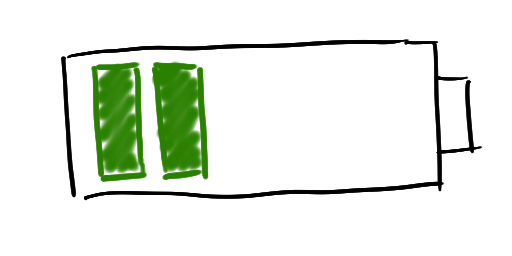
\includegraphics[scale=0.2]{images/battarie_low.png}};
		%\visible<3>{
		%\begin{tikzpicture}
		%	\node[] (i1) at (0,0) {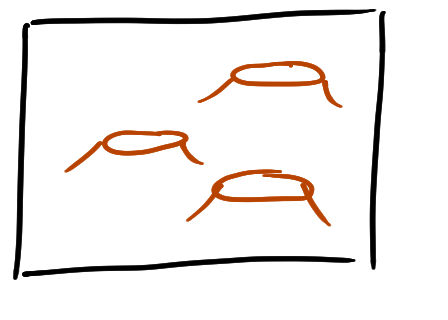
\includegraphics[scale=0.15]{images/image1.png}};
		%	\node[] (i2) at (3,0) {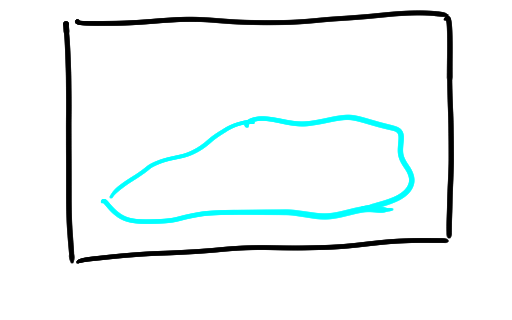
\includegraphics[scale=0.15]{images/image3.png}};
		%	\node[] (i3) at (6.2,0) {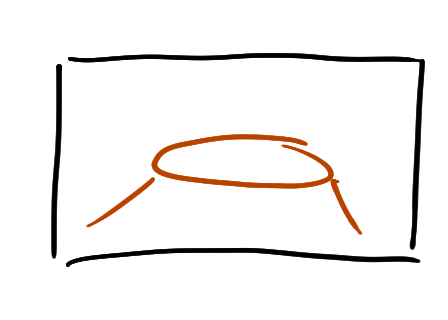
\includegraphics[scale=0.15]{images/image2.png}};
		%	\node[] (and) at (1.4,0) {\Huge $\wedge$};
		%	\node[] (and) at (4.7,0) {\Huge $\vee$};
		%	\node[] (gd) at (3,-1.7) {\huge Goal Property};
		%
		%\end{tikzpicture}
		%}


			%\node[draw, fill=mLightBrown!30] (mugs1) at (5,0) {
			%	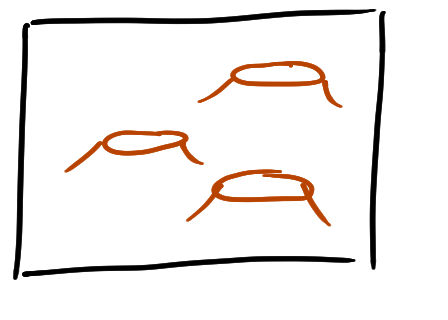
\includegraphics[scale=0.09]{images/image1.png} 
			%	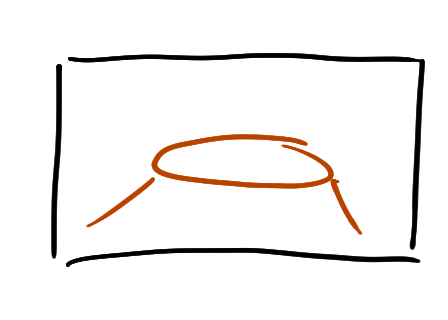
\includegraphics[scale=0.09]{images/image2.png}
			%};
			\node[draw, fill=mLightBrown!30] (mugs2) at (5,-1) {
				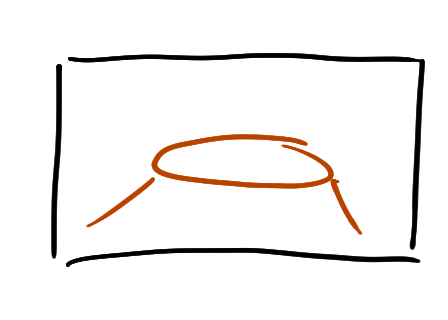
\includegraphics[scale=0.09]{images/image2.png}
				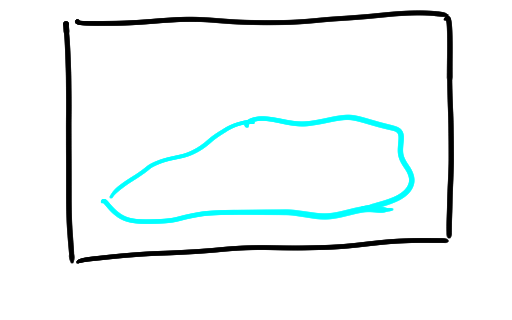
\includegraphics[scale=0.09]{images/image3.png} 
			};
		\end{tikzpicture}
	\end{center}


	\vspace*{0.3cm}
	\hrule
	\vspace*{0.5cm}
	\visible<2->{
	\large\textbf{$\plans$-Entailment}:\\
	\begin{center}
	\begin{tikzpicture}
		%\node[] (i1) at (0,0) {
		%	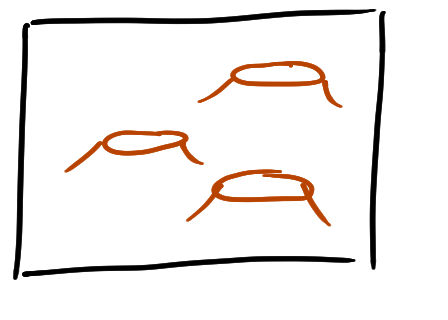
\includegraphics[scale=0.1]{images/image1.png} 
		%};
		%\node[] (i2) at (3,0) {
		%	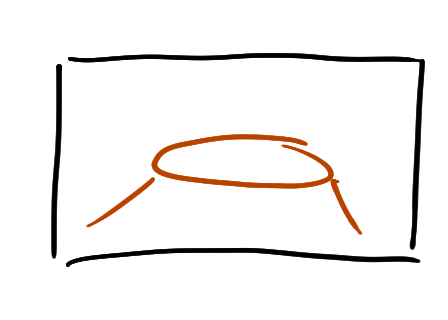
\includegraphics[scale=0.1]{images/image2.png}
		%};
		%\node[] (n1) at (3,0) {
		%	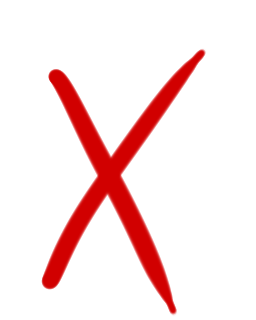
\includegraphics[scale=0.1]{images/no.png} 
		%};
		%\node[] (i22) at (0,-1.8) {
		%	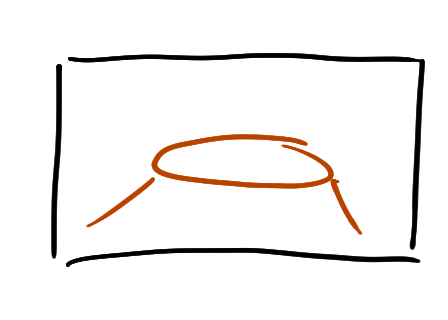
\includegraphics[scale=0.1]{images/image2.png}
		%};
		%\node[] (i12) at (3,-1.8) {
		%	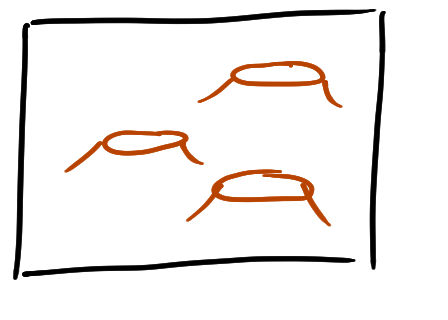
\includegraphics[scale=0.1]{images/image1.png}
		%};
		%\node[] (n2) at (3,-1.8) {
		%	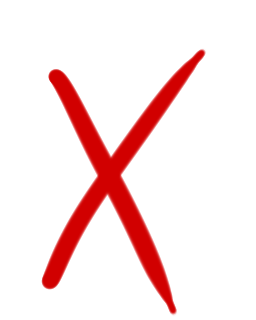
\includegraphics[scale=0.1]{images/no.png}
		%};

		%\draw[thick, ->] (i1) to (i2);
		%\draw[thick, ->] (i22) to (i12);

		\visible<2->{
		\node[] (i23) at (5,0) {
			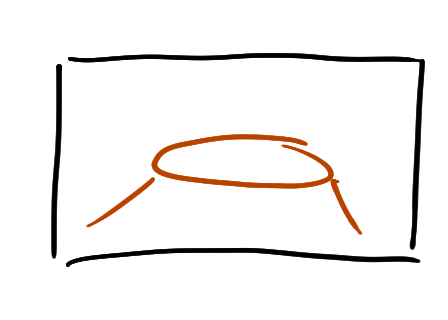
\includegraphics[scale=0.1]{images/image2.png} 
		};
		\node[] (i3) at (8,0) {
			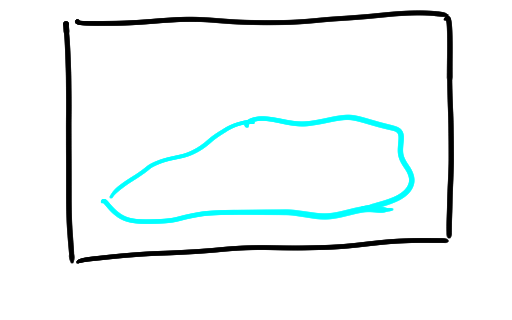
\includegraphics[scale=0.1]{images/image3.png}
		};
		\node[] (n3) at (8,0) {
			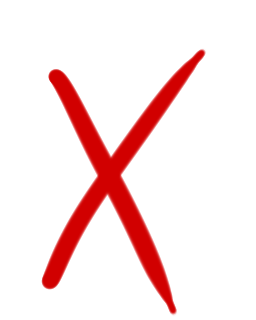
\includegraphics[scale=0.1]{images/no.png} 
		};
		\node[] (i32) at (5,-1.8) {
			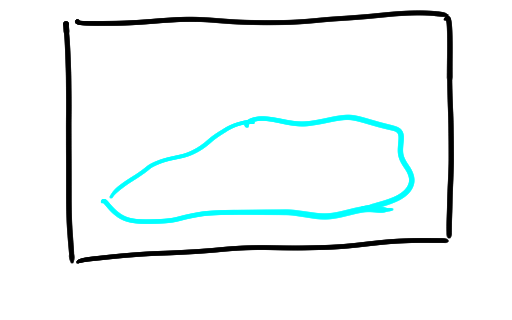
\includegraphics[scale=0.1]{images/image3.png}
		};
		\node[] (i24) at (8,-1.8) {
			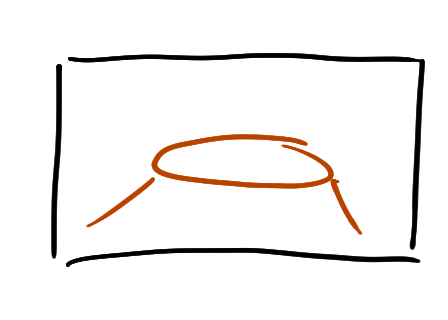
\includegraphics[scale=0.1]{images/image2.png}
		};
		\node[] (n4) at (8,-1.8) {
			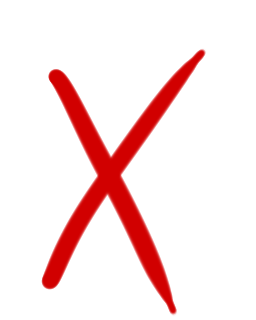
\includegraphics[scale=0.1]{images/no.png}
		};

		\draw[thick, ->] (i23) to (i3);
		\draw[thick, ->] (i32) to (i24);
		}
	\end{tikzpicture}
	}
	\end{center}

	
\end{frame}





\begin{frame}[standout]
	\Huge \textsc{Outlook}
\end{frame}

\begin{frame}{Plan-Properties: Input}
	\centering
	\begin{tikzpicture}
		\node[draw, minimum width=3.5cm, minimum height=2.5cm] (framework) at (0,0) {\Large \textbf{Framework}};

		\visible<2->{
			\node[] (task) at (-3.8,1.3) {\Large \textbf{Problem}};
			\node[] (task2) at (-4.5,2.3) {
\includegraphics[scale=0.05]{images/rover1.png}};
			\node[] (task3) at (-3.1,2.3) {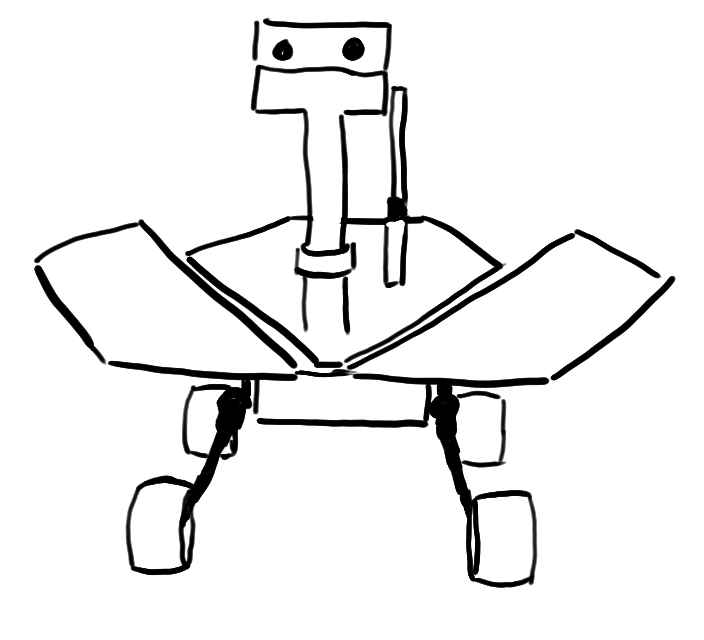
\includegraphics[scale=0.05]{images/rover2.png}};
			\node[] (task4) at (-4.5,3.3) {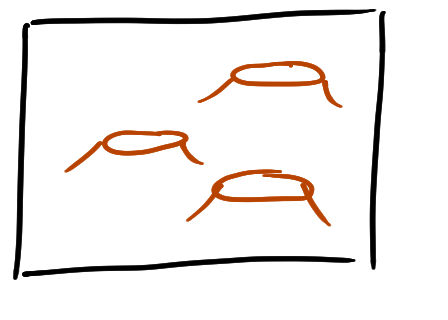
\includegraphics[scale=0.05]{images/image1.png}};
			\node[] (task5) at (-3.85,3.3) {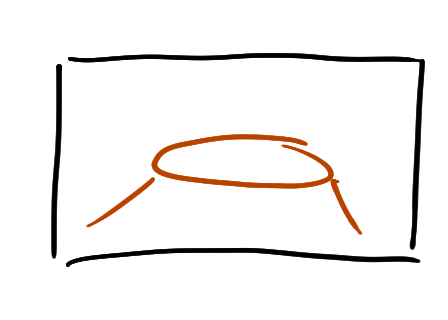
\includegraphics[scale=0.05]{images/image2.png}};
			\node[] (task6) at (-3.1,3.3) {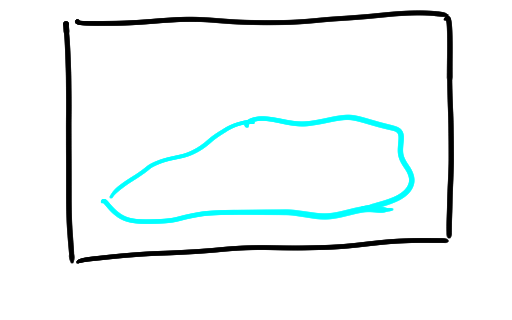
\includegraphics[scale=0.05]{images/image3.png}};
		}

		\visible<5->{
			\node[] (props) at (-3.8,-1.1) {\Large \textbf{Properties}};
			\node[draw, inner sep=1pt] (props1) at (-4.6,-2.5) {
				\resizebox{!}{1.2cm}{%
					\dontuseconnection{1}{1}{2}
				}
			};
			\node[draw, inner sep=1pt] (props2) at (-2.8,-2.5) {
				\resizebox{!}{1.2cm}{%
					\specificrover{1}{1}
				}
			};
		}
		\visible<6->{
			\node[] (no) at (-3.8,-1.8) {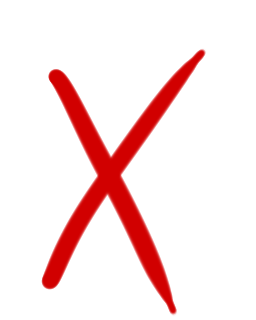
\includegraphics[scale=0.3]{images/no.png}};
		}

		\visible<3->{
			\node[] (plan) at (3.8,1.3) {\Large \textbf{Plan}};
			\node[draw, align=left, fill=white] (plan2) at (4,3.0) {
					\scriptsize
					$drive(R_1,L_1,L2)$\\[-0.2cm]
					\scriptsize
					$takeImage_1(R_1)$\\[-0.2cm]
					\scriptsize
					$drive(R_2,L_4,L_5)$\\[-0.2cm]
					\scriptsize
					$takeImage_3(R_2)$\\[-0.2cm]
					\scriptsize
					$drive(R_2,L_5,L_6)$\\[-0.2cm]
					\scriptsize
					$\cdots$
			};
		}

		\visible<4->{
			\node[] (exp) at (3.8,-1.3) {\Large \textbf{Explanation}};
			\node[] (exp2) at (3.8,-2.5) {
				\resizebox{!}{1cm}{%
				\begin{tikzpicture}
					\node[draw] (p1) at (5,0) {
						\specificrover{1}{1}
					};

					\node[draw] (p4) at (0,0) {
						\dontuseconnection{1}{1}{2}
					};
					\node[] (not) at (5,0) {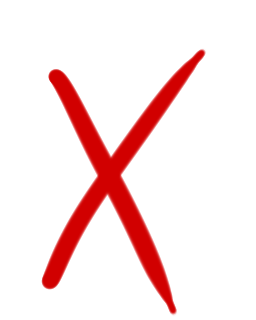
\includegraphics[scale=0.3]{images/no.png}};

					\draw[thick, ->] (p4) to (p1);
				\end{tikzpicture}
				}
			};
		}

		\draw[->, line width=2pt] (-4,0) to (-2.5,0);
		\draw[->, line width=2pt] (2.5,0) to (4,0);

	\end{tikzpicture}
\end{frame}

\begin{frame}{Plan-Properties: Languages}
\centering
\begin{tikzpicture}
	\node[] (p1) at (-0.5,-3.5) {\samerover{1}{2}};
	\node[draw,inner sep=2pt] (p2) at (3,-3.5) {\orderprop{1}{2}};
	\node[draw,inner sep=2pt] (p3) at (6.5,-3.5) {\energylimit{1}};
	\node[] (p4) at (-0.5,0) {\specificrover{1}{2}};
	\node[] (p5) at (3,0) {\useconnection{1}{x}{y}};
	\node[] (p6) at (6.5,0) {\dontuseconnection{1}{x}{y}};
\end{tikzpicture}
\end{frame}

\begin{frame}{Iterative Planning}
	\centering
	%\begin{tikzpicture}
	%	\visible<2->{\node[draw, fill=blue!30] at (5.8,0) {Here is your $plan$.};}
	%	\visible<3->{\node[draw, fill=mLightGreen!30] at (-0.1,-1.2) {Why don't you avoid connection X ?};}
	%	\visible<4->{\node[draw, fill=blue!30, align=left] at (4.1,-2.4) {Because you would not be able to take\\ all image using a single rover.};}
	%	\visible<5->{\node[draw, fill=mLightGreen!30] at (0,-3.6) {I don't care about using more rovers.};}
	%	\visible<6->{\node[draw, fill=blue!30, align=left] at (4.6,-4.8) {Here is a new $plan'$ using two\\ rovers but avoiding connection X.};}
	%\end{tikzpicture}
	\begin{tikzpicture}
		\visible<1>{\node[] (i1) at (0,0) {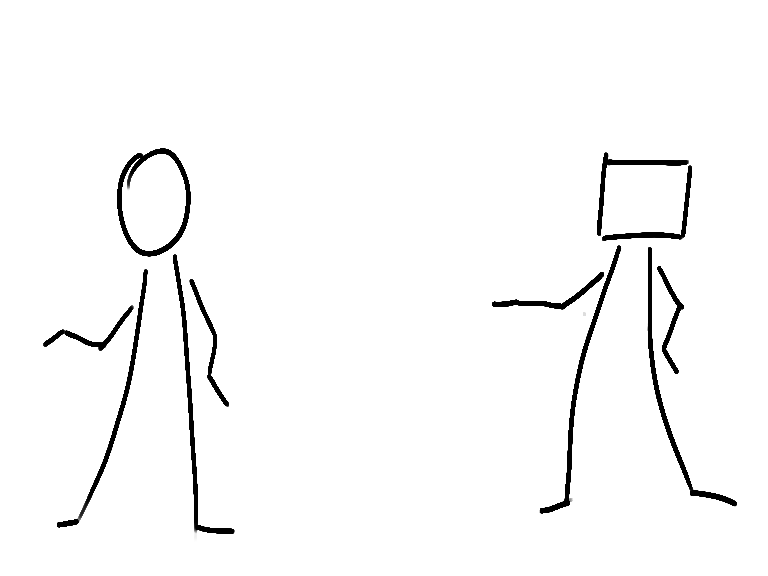
\includegraphics[scale=0.30]{images/iter/iter1.png}};}
		\visible<2>{\node[] (i2) at (0,0) {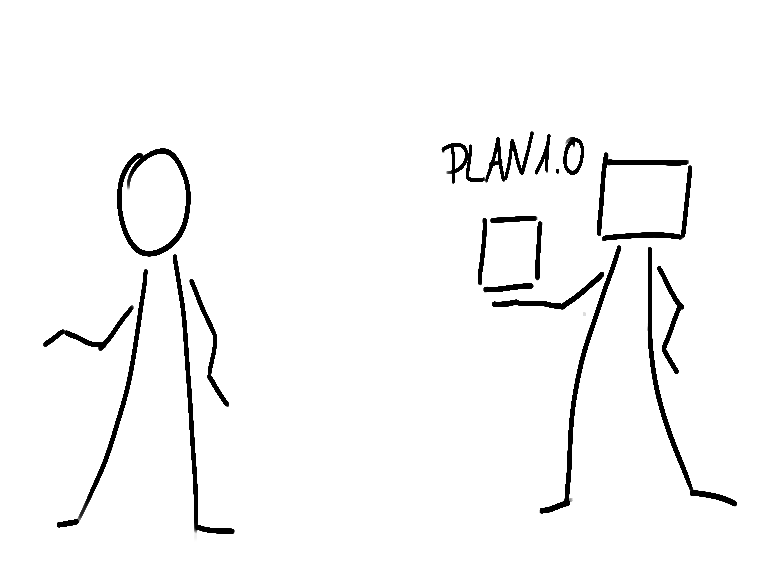
\includegraphics[scale=0.30]{images/iter/iter2.png}};}
		\visible<3>{\node[] (i3) at (0,0) {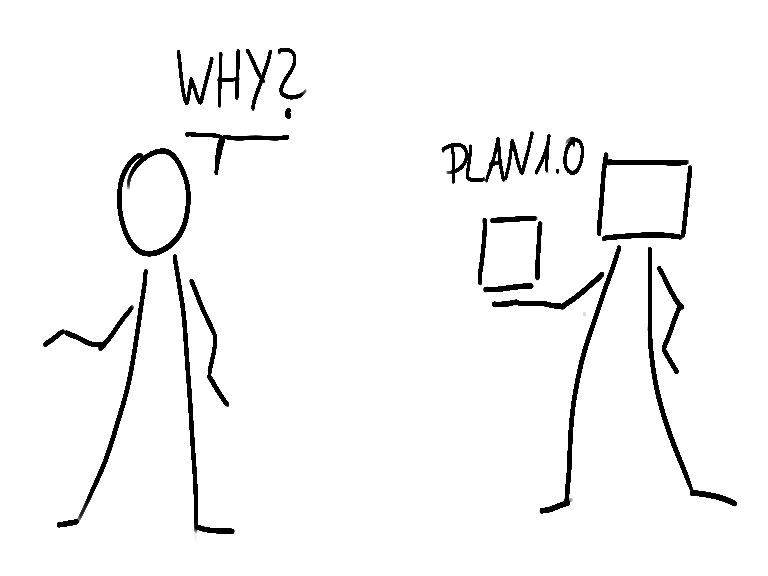
\includegraphics[scale=0.30]{images/iter/iter3.png}};}
		\visible<4>{\node[] (i4) at (0,0) {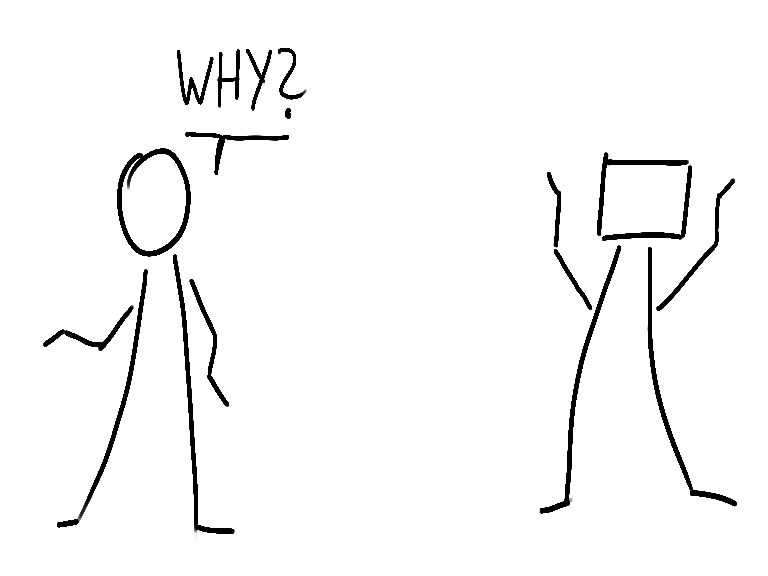
\includegraphics[scale=0.30]{images/iter/iter4.png}};}
		\visible<4-5>{\node[] (i4) at (2.8,2.3) {
			\resizebox{!}{1.5cm}{%
			\begin{tikzpicture}
				\node[draw] (p1) at (5,0) {
					\specificrover{1}{1}
				};

				\node[draw] (p4) at (0,0) {
					\dontuseconnection{1}{1}{2}
				};
				\node[] (not) at (5,0) {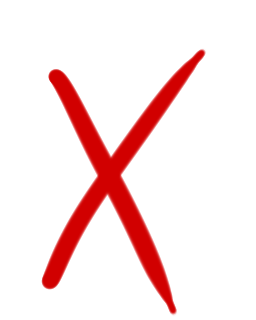
\includegraphics[scale=0.3]{images/no.png}};

				\draw[thick, ->] (p4) to (p1);
			\end{tikzpicture}
			}
		};}
		\visible<5>{\node[] (i5) at (0,0) {\includegraphics[scale=0.30]{images/iter/iter5.png}};}
		\visible<6>{\node[] (i6) at (0,0) {\includegraphics[scale=0.30]{images/iter/iter6.png}};}
	\end{tikzpicture}\\

\end{frame}


\begin{frame}{Why?}
	\centering
	\begin{tikzpicture}
		\node[] (p) at (3,1) {
			\resizebox{!}{2cm}{%
			\begin{tikzpicture}
				\node[draw] (p1) at (5,0) {
					\specificrover{1}{1}
				};

				\node[draw] (p4) at (0,0) {
					\dontuseconnection{1}{1}{2}
				};
				\node[] (not) at (5,0.9) {\includegraphics[scale=0.1]{images/no.png}};

				\draw[thick, ->] (p4) to (p1);
				\visible<5->{
					\node[] (no) at (2.5,0) {\includegraphics[scale=0.1]{images/no.png}};
				}
			\end{tikzpicture}
			}
		};
		
		\node[] (ai_exp) at (3,-2) {\includegraphics[scale=0.2]{images/ai_exp.png}};

		\visible<2>{
			\node[] (child_why) at (-3,-1.0) {\includegraphics[scale=0.22]{images/warum_darum.png}};
		}

		\visible<3>{
			\node[draw] (pa) at (-3,-1.5) {
				\energylimitloc{1}
			};
		}
		\visible<4->{
		\node[] (pa) at (-3,-1.5) {
			\begin{tikzpicture}
				\node[] (task1) at (-4.5,4.0) {\Large Planning Task};
				\node[] (task2) at (-4.9,1.8) {\includegraphics[scale=0.07]{images/rover1.png}};
				\node[] (task3) at (-2.8,1.8) {\includegraphics[scale=0.07]{images/rover2.png}};
				\node[] (task4) at (-4.7,3.3) {\includegraphics[scale=0.07]{images/image1.png}};
				\node[] (task5) at (-3.85,3.3) {\includegraphics[scale=0.07]{images/image2.png}};
				\node[] (task6) at (-2.8,3.3) {\includegraphics[scale=0.07]{images/image3.png}};
				\node[] (task7) at (-3.8,0.7) {\includegraphics[scale=0.1]{images/battarie.png}};
				\visible<5->{
					\node[] (task7) at (-3.8,0.7) {\includegraphics[scale=0.1]{images/no.png}};
				}
			\end{tikzpicture}
		};
		}
	\end{tikzpicture}\\

\end{frame}

\begin{frame}[plain]
	\centering
	\begin{tikzpicture}
		\node[draw, minimum width=3.5cm, minimum height=2.5cm] (framework) at (0,0) {\Large \textbf{Framework}};

		\node[] (task) at (-3.8,1.3) {\Large \textbf{Problem}};
		\node[] (task2) at (-4.5,2.3) {\includegraphics[scale=0.05]{images/rover1.png}};
		\node[] (task3) at (-3.1,2.3) {\includegraphics[scale=0.05]{images/rover2.png}};
		\node[] (task4) at (-4.5,3.3) {\includegraphics[scale=0.05]{images/image1.png}};
		\node[] (task5) at (-3.85,3.3) {\includegraphics[scale=0.05]{images/image2.png}};
		\node[] (task6) at (-3.1,3.3) {\includegraphics[scale=0.05]{images/image3.png}};

		\node[] (props) at (-3.8,-1.1) {\Large \textbf{Properties}};
		\node[draw, inner sep=1pt] (props1) at (-4.6,-2.5) {
			\resizebox{!}{1.2cm}{%
				\dontuseconnection{1}{1}{2}
			}
		};
		\node[draw, inner sep=1pt] (props2) at (-2.8,-2.5) {
			\resizebox{!}{1.2cm}{%
				\specificrover{1}{1}
			}
		};

		%\node[] (no) at (-3.8,-1.8) {\includegraphics[scale=0.3]{images/no.png}};

		\node[] (plan) at (3.8,1.3) {\Large \textbf{Plan}};
		\node[draw, align=left, fill=white] (plan2) at (4,3.0) {
				\scriptsize
				$drive(R_1,L_1,L2)$\\[-0.2cm]
				\scriptsize
				$takeImage_1(R_1)$\\[-0.2cm]
				\scriptsize
				$drive(R_2,L_4,L_5)$\\[-0.2cm]
				\scriptsize
				$takeImage_3(R_2)$\\[-0.2cm]
				\scriptsize
				$drive(R_2,L_5,L_6)$\\[-0.2cm]
				\scriptsize
				$\cdots$
		};

		\node[] (exp) at (3.8,-1.3) {\Large \textbf{Explanation}};
		\node[] (exp2) at (3.8,-2.5) {
			\resizebox{!}{1cm}{%
			\begin{tikzpicture}
				\node[draw] (p1) at (5,0) {
					\specificrover{1}{1}
				};

				\node[draw] (p4) at (0,0) {
					\dontuseconnection{1}{1}{2}
				};
				\node[] (not) at (5,0) {\includegraphics[scale=0.3]{images/no.png}};

				\draw[thick, ->] (p4) to (p1);
			\end{tikzpicture}
			}
		};

		\draw[->, line width=2pt] (-4,0) to (-2.5,0);
		\draw[->, line width=2pt] (2.5,0) to (4,0);

	\end{tikzpicture}

\end{frame}






\end{document}


